\documentclass{article}
\usepackage{graphicx}
\usepackage{subcaption}
\usepackage{geometry}
 \geometry{
 a4paper,
 total={170mm,257mm},
 left=20mm,
 top=20mm,
 }

\title{Assignment 2 - Part 3.1: The Filter Gallery \\ Feature Extraction \& Visual Interpretability}
\date{February 12, 2026}

\begin{document}

\maketitle

\section{Introduction}
This experiment investigates "The Filter Gallery" to understand how Convolutional Neural Networks (CNNs) "see" the world compared to Fully Connected Neural Networks (FCNNs). We extract and visualize the learned weights of the first layer from models trained on MNIST and Tiny-ImageNet-10. This visualization highlights the difference between the spatially invariant local features learned by CNNs and the global templates learned by FCNNs.

\section{Methodology}

\subsection{Architectures}
We implemented two architectures:
\begin{itemize}
    \item \textbf{SimpleCNN:} A 2-layer CNN.
    \begin{itemize}
        \item Layer 1: Conv2d (16 filters, $3\times3$) $\rightarrow$ ReLU $\rightarrow$ MaxPool ($2\times2$)
        \item Layer 2: Conv2d (32 filters, $3\times3$) $\rightarrow$ ReLU $\rightarrow$ MaxPool ($2\times2$)
        \item Classifier: Fully Connected Layer
    \end{itemize}
    \item \textbf{FCNN } A 3-layer Fully Connected Network.
    \begin{itemize}
        \item Input: $28\times28 \rightarrow 128$ (ReLU)
        \item Hidden 1: $128 \rightarrow 128$ (ReLU)
        \item Hidden 2: $128 \rightarrow 128$ (ReLU)
        \item Output: $128 \rightarrow 10$
    \end{itemize}
\end{itemize}

\subsection{Datasets}
\begin{itemize}
    \item \textbf{MNIST:} Grayscale digits ($28\times28$).
    \item \textbf{Tiny-ImageNet-10:} Color images ($64\times64$, 3 channels) from 10 selected classes.
\end{itemize}

\section{Results \& Visualizations}

\subsection{CNN Filters (MNIST)}
The first layer of the CNN sees the input image locally. The visualized filters (Figure \ref{fig:cnn_mnist}) resemble \textbf{Gabor filters}, acting as basic edge, corner, and texture detectors. They do not look like digits themselves, but rather the building blocks of digits.

\begin{figure}[h]
    \centering
    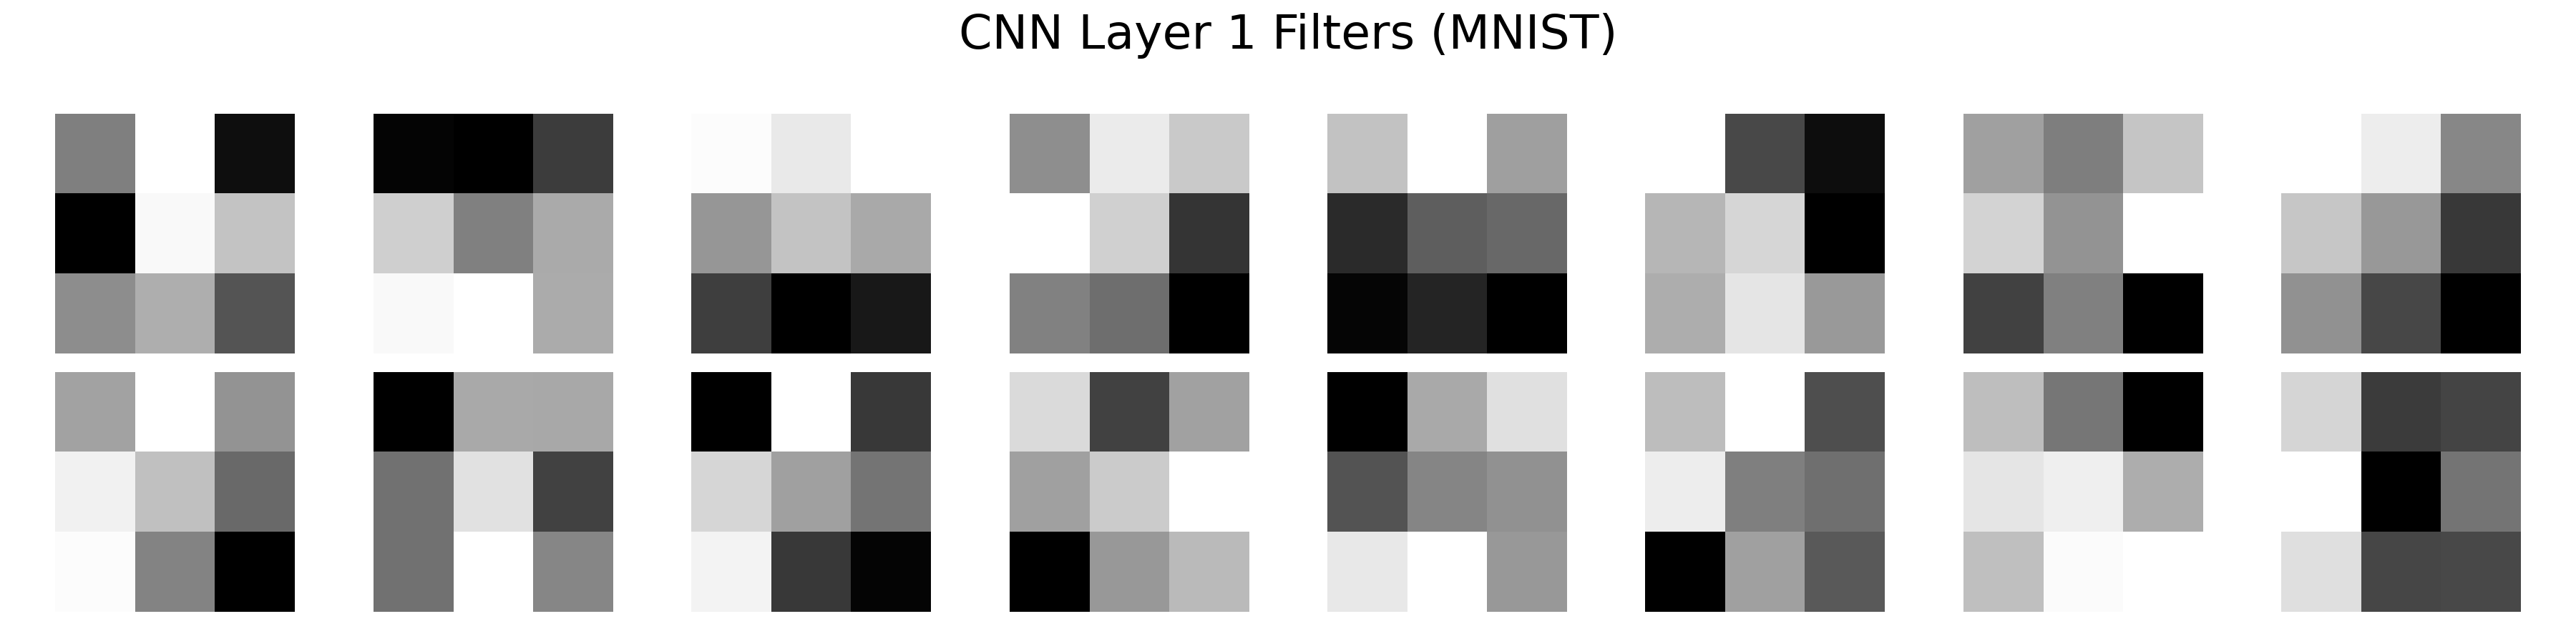
\includegraphics[width=0.8\textwidth]{plots/cnn_mnist_filters.png}
    \caption{First Layer Convolutional Kernels of SimpleCNN on MNIST. Notice the simple edge and texture patterns.}
    \label{fig:cnn_mnist}
\end{figure}

\subsection{CNN Filters (Tiny-ImageNet-10)}
For the color dataset, the kernels operate on 3 input channels (RGB). Figure \ref{fig:cnn_tiny} shows these filters. They have evolved into not just edge detectors but also \textbf{color blobs} and \textbf{chromatic edge detectors}. This demonstrates the network's ability to learn spatial and chromatic primitives early in the hierarchy.

\begin{figure}[h]
    \centering
    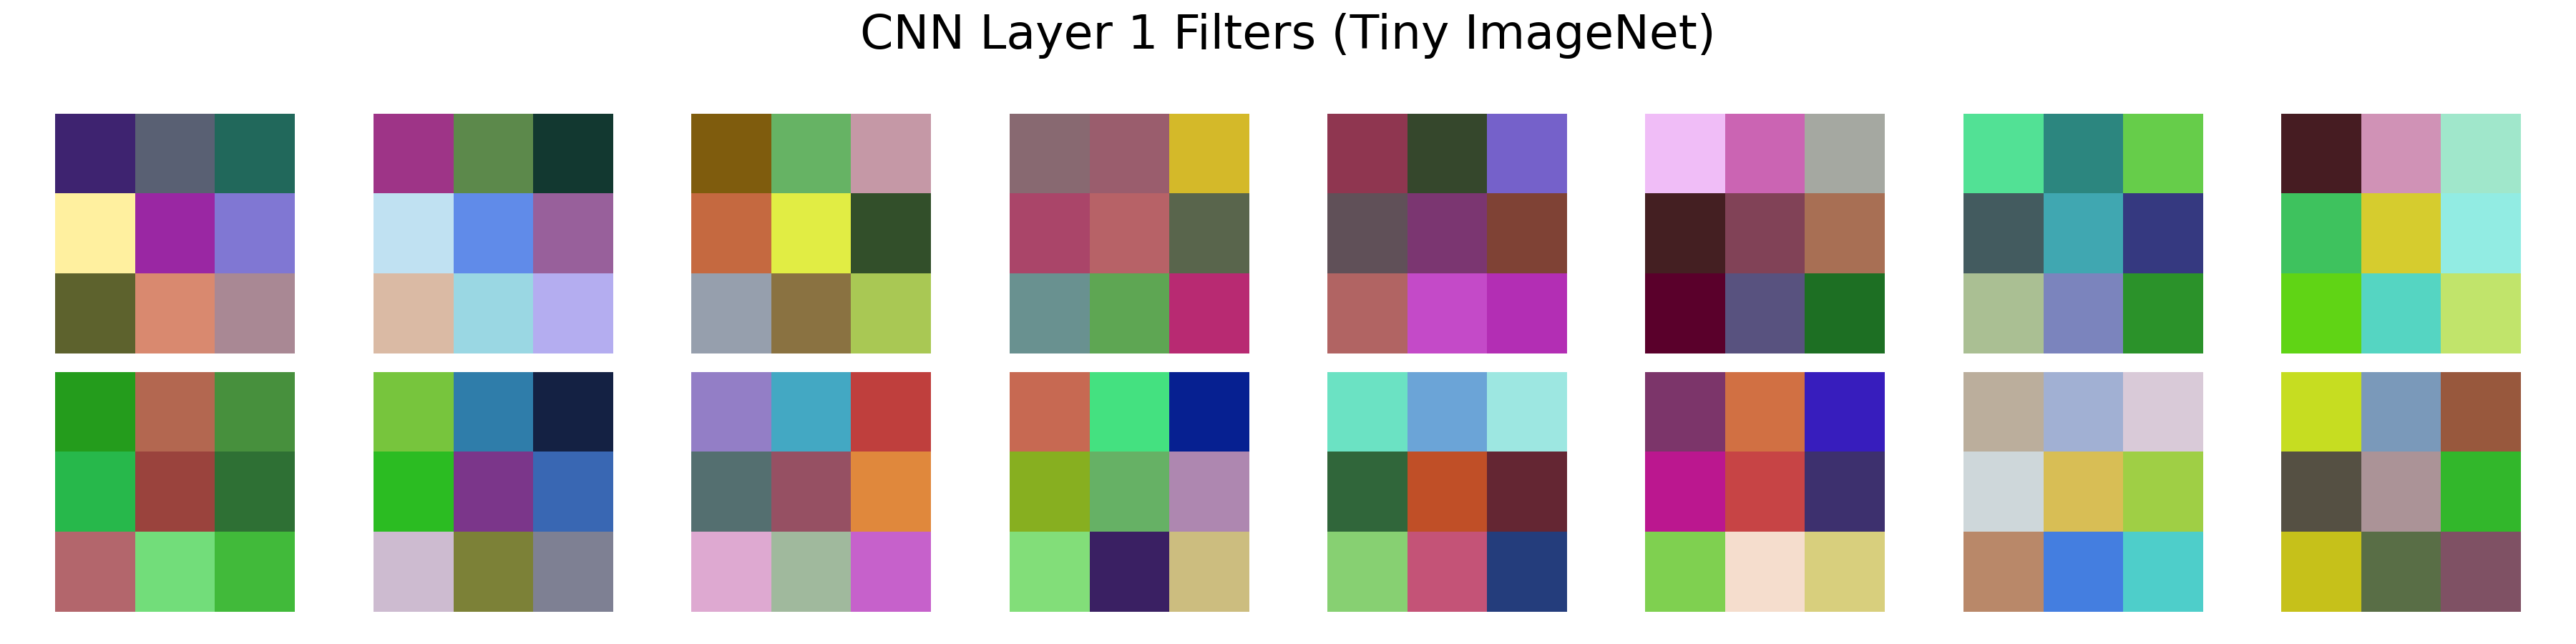
\includegraphics[width=0.8\textwidth]{plots/cnn_tiny_filters.png}
    \caption{First Layer Convolutional Kernels of SimpleCNN on Tiny-ImageNet. The filters capture color gradients and edges.}
    \label{fig:cnn_tiny}
\end{figure}

\subsection{FCNN Weights Comparison}
In contrast to the CNN, the weights of the input layer of the FCNN (Figure \ref{fig:fcnn}) map specific pixels to hidden neurons.

\begin{figure}[h]
    \centering
    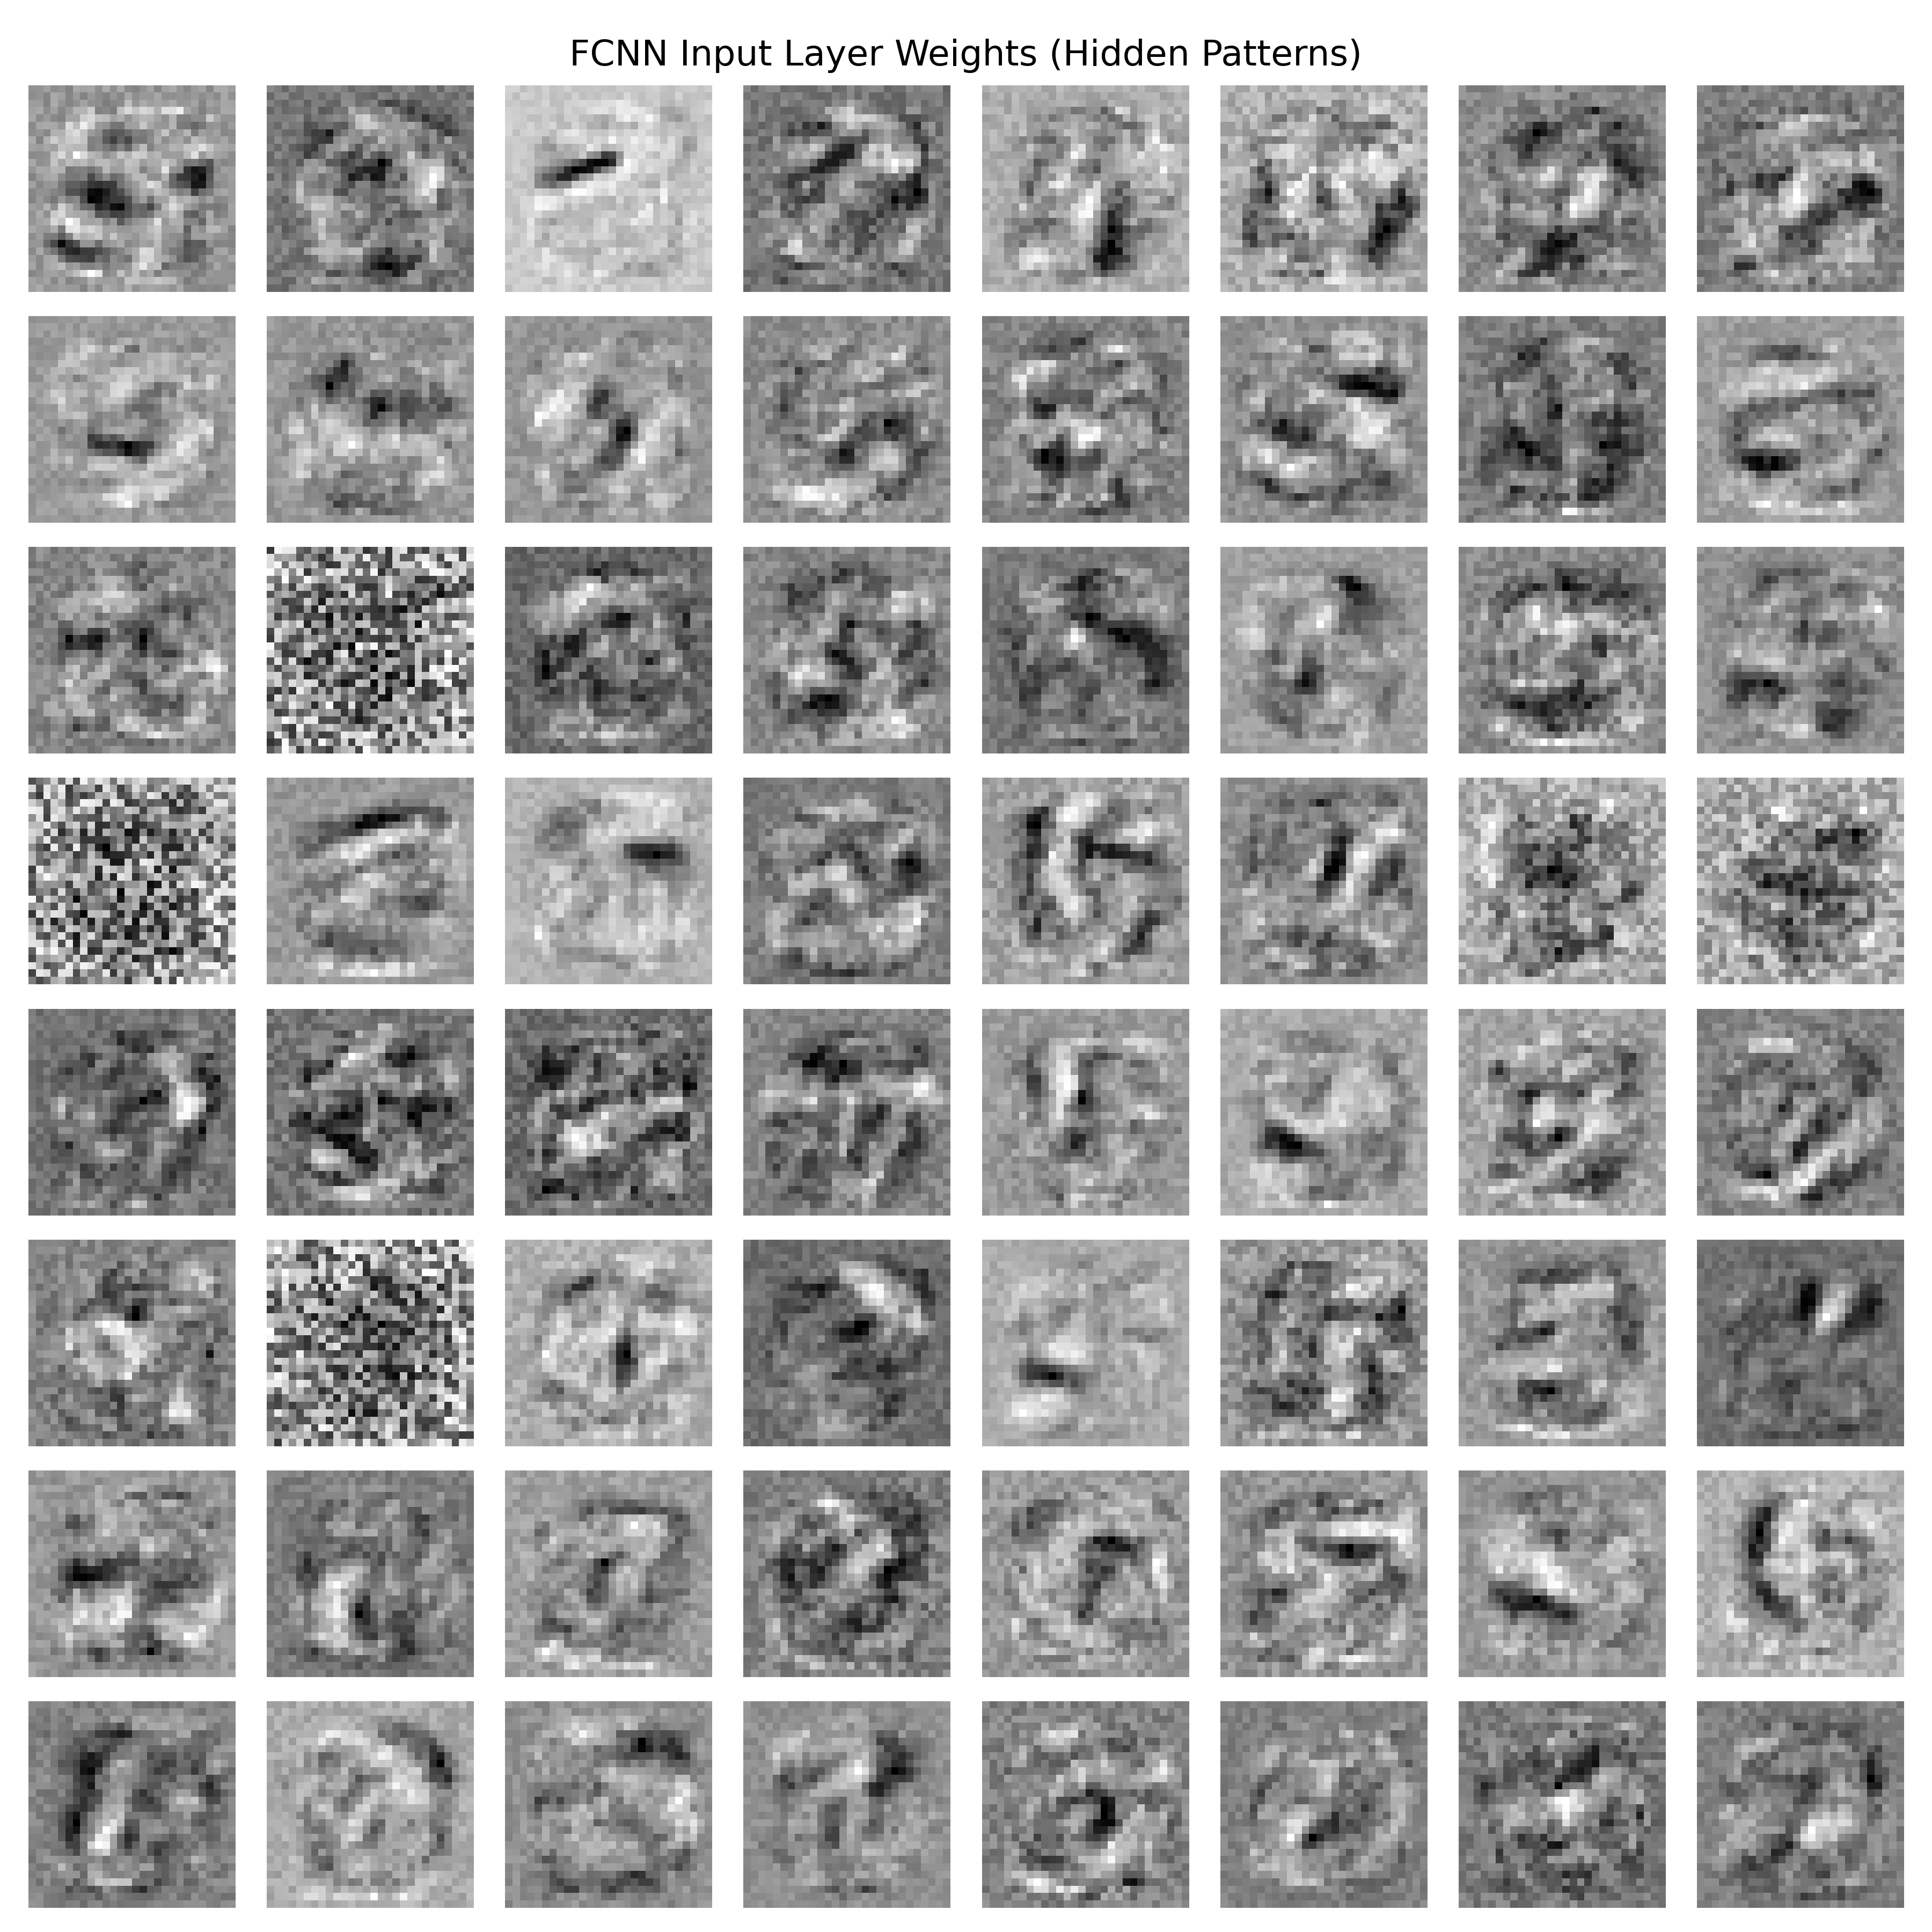
\includegraphics[width=0.8\textwidth]{plots/fcnn_mnist_weights.png}
    \caption{Input Layer Weights of the FCNN on MNIST. These represent the "feature detectors" for the first hidden layer.}
    \label{fig:fcnn}
\end{figure}

\section{Analysis}
\begin{enumerate}
    \item \textbf{CNN Filters}: Show local features like edges, corners, and color blobs (Gabor-like). They are spatially invariant and look for specific textures.
    \item \textbf{FCNN Weights}: The input layer weights of the FCNN map each pixel to a hidden neuron. These can be interpreted as templates or "feature detectors" that the hidden layer looks for. Unlike the CNN which shares filters, each neuron here looks at the whole image with fixed weights.
\end{enumerate}

\end{document}
